\documentclass[10pt,a4paper,twocolumn]{article}
\usepackage[utf8]{inputenc}
\usepackage[T1]{fontenc}
\usepackage[spanish]{babel}
\usepackage{amsmath}
\usepackage{amsfonts}
\usepackage{amssymb}
\usepackage{graphicx}
\usepackage{hyperref}
\usepackage[width=18.00cm, height=26.00cm]{geometry}
\title{Laboratorio 4\\Algoritmos}
\author{Gabriel Octavio Lozano Pinzón}

\begin{document}
	\maketitle
	\section{Obtener las mejores empresas para invertir}	
	Deseamos escoger las empresas que nos darían la mayor ganancia si invirtieramos en ella en un tiempo anterior. Para este ejercicio manejamos $6$ meses y $2$ años. Esta tarea es una tarea repetitiva y monotona si se usan medios usuales como Yahoo Finance. Se puede simplificar bastantes usando un algoritmo en Quantopian que nos permitiría automatizar esta tarea para cualquier intervalo de tiempo y analizar el crecimiento de todas las empresas para las que hay información disponible al mismo tiempo.\\
	Para resolver la tarea usamos un Notebook en los servicios provistos por Quantopian subido a github en el link \url{https://github.com/Matematikoi/Algoritmos_2020_I/blob/master/lab_4/get%20all%20stocks.ipynb}\\
		Esto nos permite obtener las mejores empresas para invertir, para el caso de 6 meses tenemos
		\begin{center}
			\begin{tabular}{ |c|c| } 
				\hline
				Empresa & Ratio de Cambio\\
				\hline
				AXSM & 322\%\\ 
				AUPH & 280\%\\ 
				\hline
			\end{tabular}
		\end{center}
		Para el caso de 2 años se tiene los siguientes resultados: 
		\begin{center}
			\begin{tabular}{ |c|c| } 
				\hline
				Empresa & Ratio de Cambio\\
				\hline
				RETA & 783\%\\ 
				AMD & 448\%\\ 
				\hline
			\end{tabular}
		\end{center}
		Estos resultados cambian un poco cuando se aplican el Hello World de Quantopian. Además los resultados dan el retorno en vez del ratio de cambio que definí como la razón entre el stock en el presente y el stock del pasado. Para el caso de AMD los resultados se observan en la Figura \ref{fig:amd}.
		\begin{figure}
			\centering
			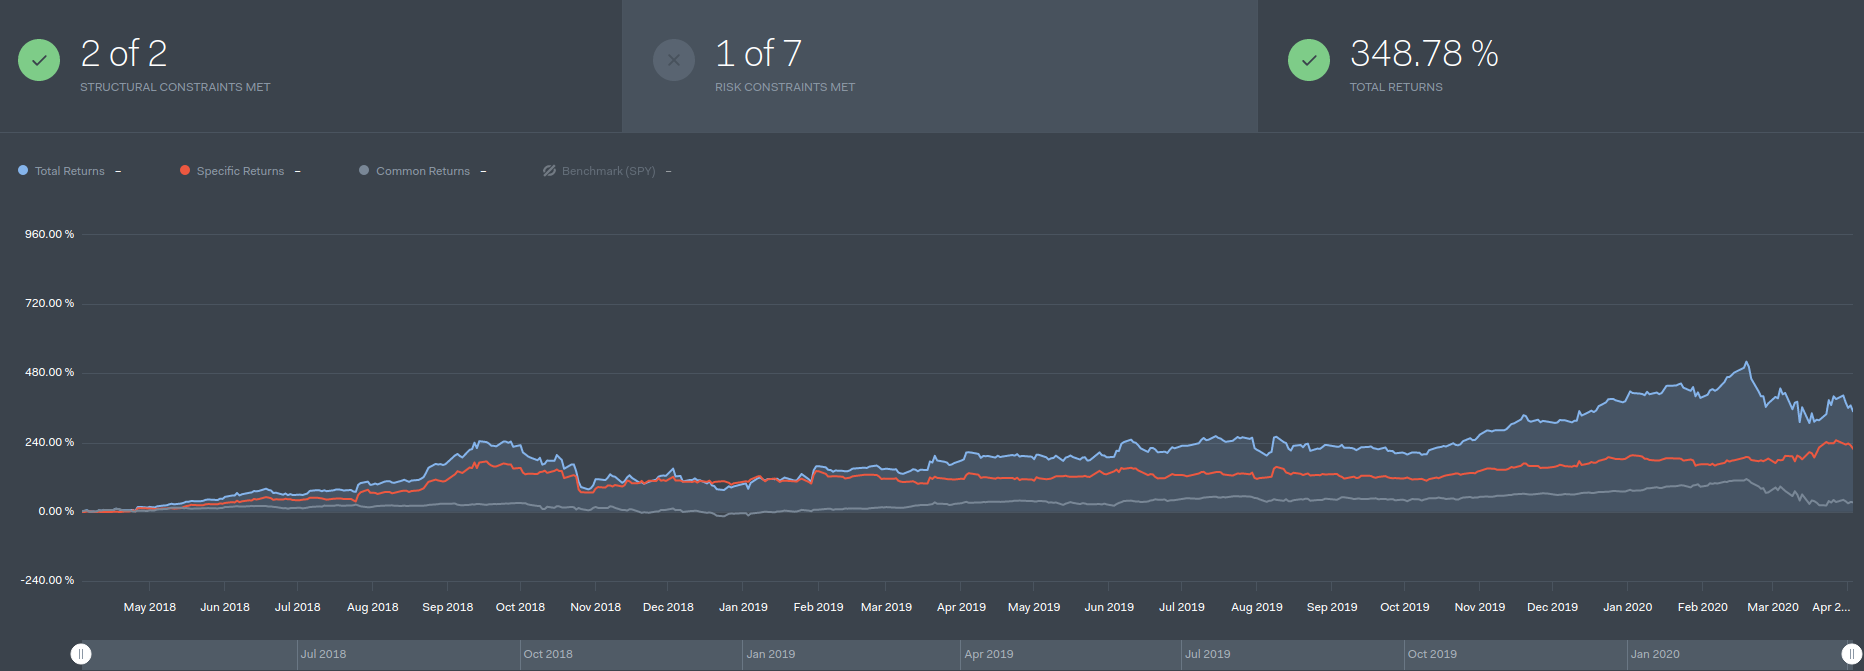
\includegraphics[width=1.0\linewidth]{amd.png}
			\caption{Resultados de invetir a $2$ años en AMD desde el $4$ de Abril de $2018$.}
			\label{fig:amd}
		\end{figure}
		\\
		También están los resultados de RETA ó Reata Pharmaceuticals, Inc. que tienen un ratio de cambio de $783\% $ pero que en quantopian no dan tan buenos resultados mostrando un retorno de solo $422\% $  como lo indica la Figura \ref{fig:reta}.\\
	
		\begin{figure}
			\centering
			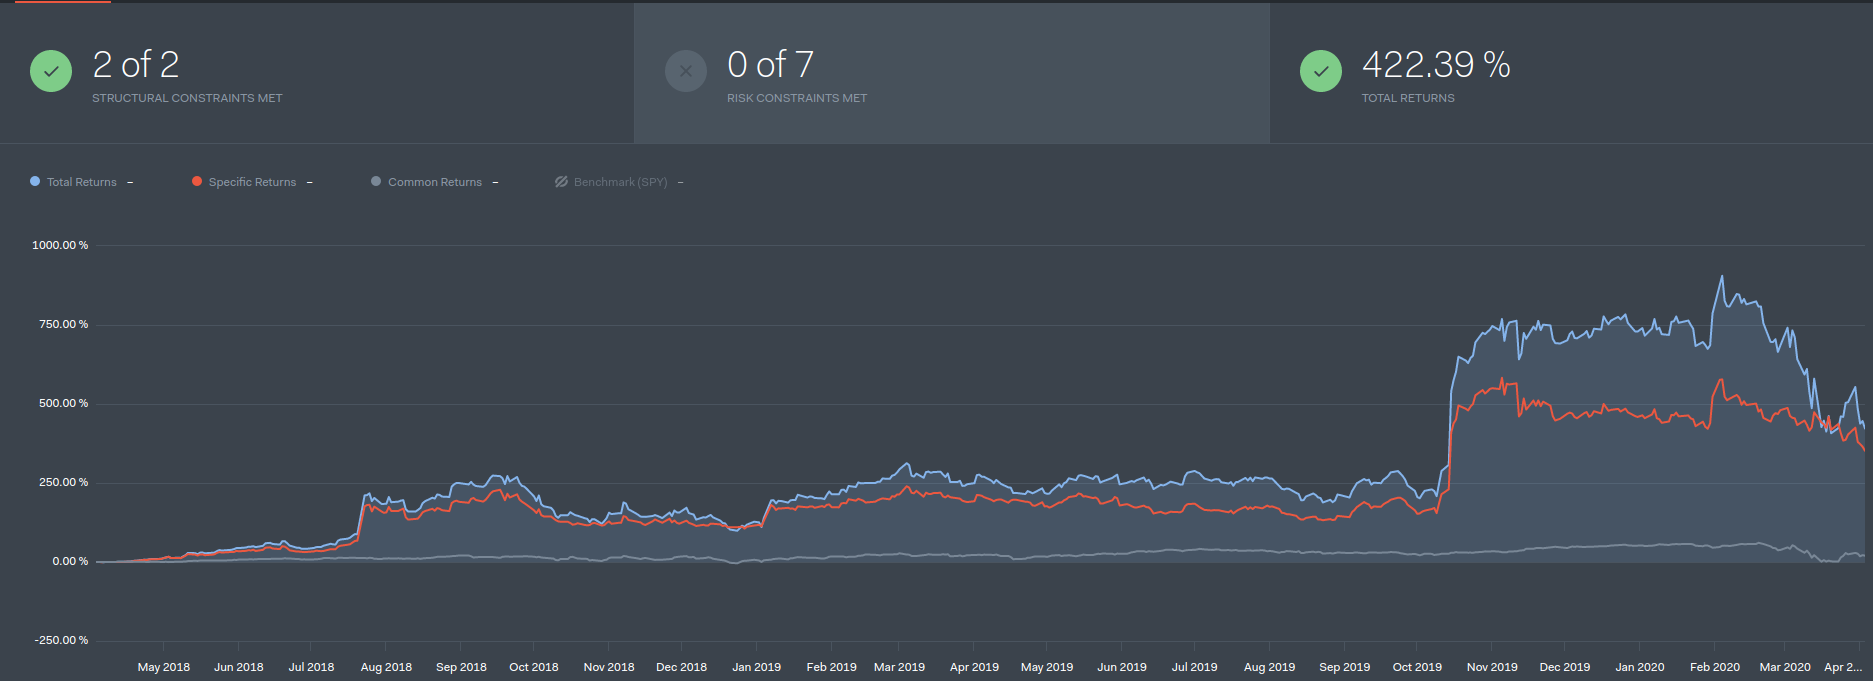
\includegraphics[width=1.0\linewidth]{RETA}
			\caption{Resultados de invertir a 2 años en RETA desde el 4 de abril del 2018.}
			\label{fig:reta}
		\end{figure}
	Pasando a las empresas con mejores Ratio de Cambio en los ultimos 6 meses tomamos primero AXSM - Axsome Therapeutics, Inc.  Los resultados para su inversión en los últimos 6 meses lo podemos observar en la Figura \ref{fig:axsm}. Similarmente para AUPH - Aurinia Pharmaceuticals Inc. podemos ver los resultados de la inversión en los últimos 6 meses en la Figura \ref{fig:auph}.\\
	
	\begin{figure}
		\centering
		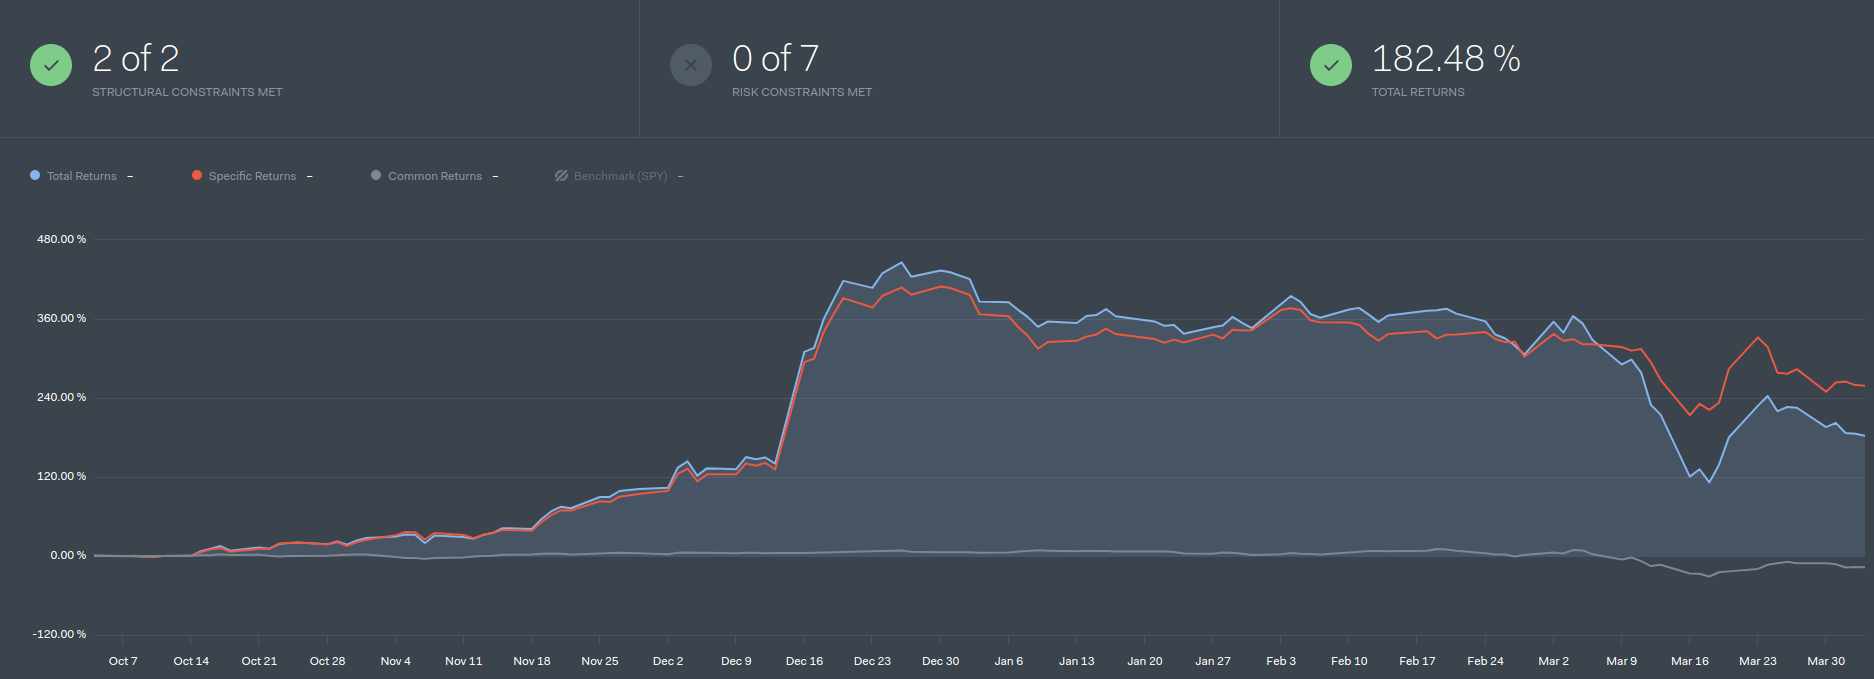
\includegraphics[width=1\linewidth]{AXSM}
		\caption{Resultados de invertir 6 meses en AXSM desde el 4 de octubre del 2019.}
		\label{fig:axsm}
	\end{figure}
	\begin{figure}
		\centering
		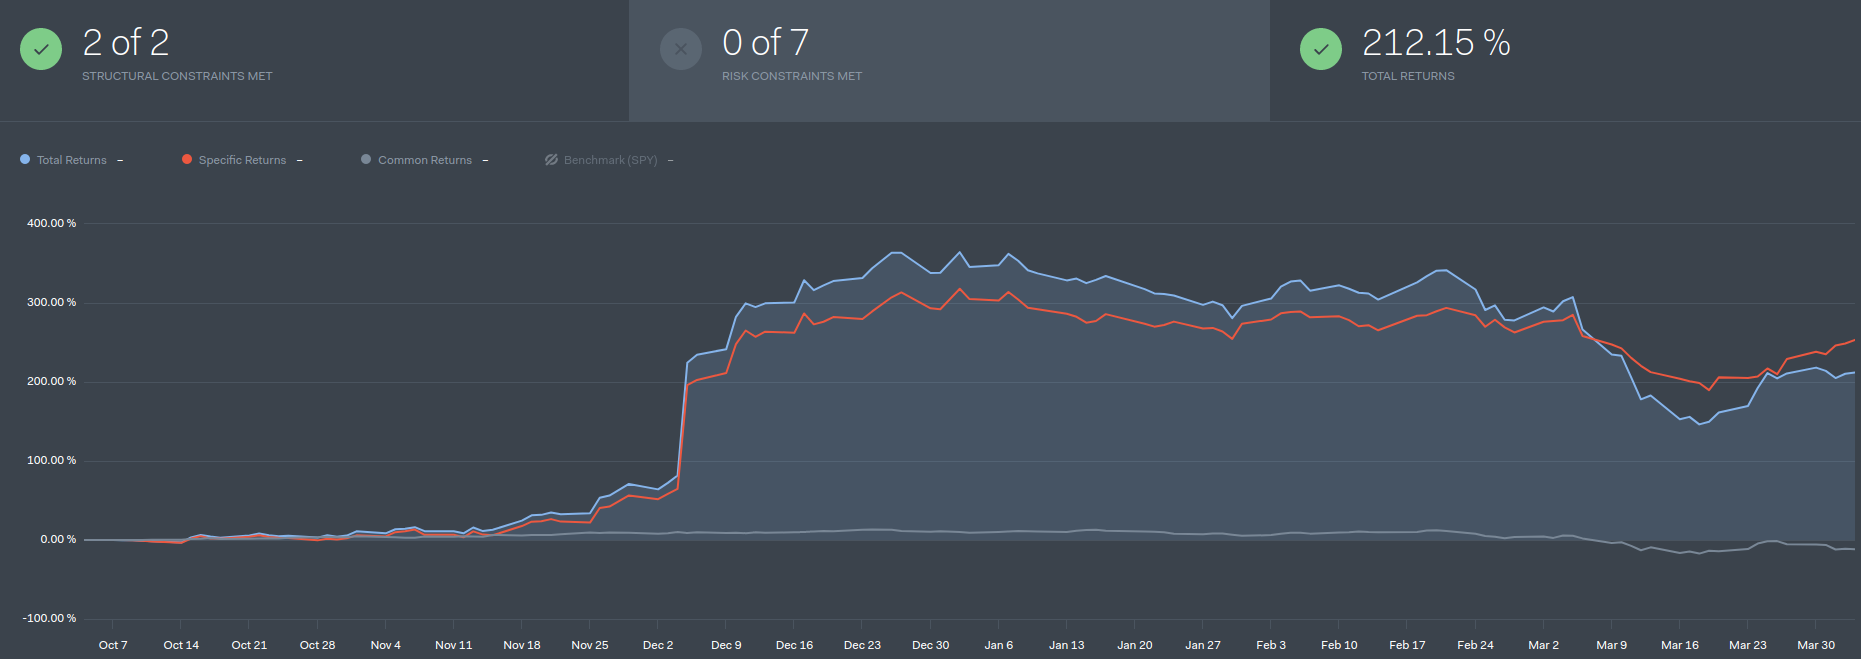
\includegraphics[width=1\linewidth]{auph}
		\caption{Resultados de invertir 6 meses en AUPH desde el 4 de octubre del 2019.}
		\label{fig:auph}
	\end{figure}
	Hay que notar que en épocas más normales los retornos teniendo una predicción de este tipo van a ser más altas pero en este preciso momento ha habido un desplome en la bolsa y la mayoría de empresas se han visto afectadas por ella. Incluso nuestras empresas con mejor ratio de cambio han sido afectadas en los ultimos meses por la pandemia. Esto se ha reflejado en el precio de sus acciones. 
		
	\end{document}
	
	
	
	
	
	
